%Este trabalho está licenciado sob a Licença Creative Commons Atribuição-CompartilhaIgual 3.0 Não Adaptada. Para ver uma cópia desta licença, visite http://creativecommons.org/licenses/by-sa/3.0/ ou envie uma carta para Creative Commons, PO Box 1866, Mountain View, CA 94042, USA.

%\documentclass[main.tex]{subfiles}
%\begin{document}

\chapter{Aritmética de máquina}\index{aritmética!de máquina}

\section{Sistema de numeração e mudança de base}\index{mudança de base}\index{sistema de numeração}
Usualmente, utilizamos o sistema de numeração decimal para representar números. Esse é um sistema de numeração posicional onde a posição do dígito indica a potência de $10$ que o dígito está representando.

\begin{ex}
  O número $293$ é decomposto como
  \begin{equation*}
    \begin{split}
      293 &= 2\ \hbox{centenas}+9\ \hbox{dezenas}+3\ \hbox{unidades}\\
      &= 2\times 10^2+9\times 10^1+3\times 10^0.      
    \end{split}
  \end{equation*}
\end{ex}

O sistema de numeração posicional também pode ser usado com outras bases. Vejamos a seguinte definição.

\begin{defn}[Sistema de numeração de base $b$]\label{def:sistema_de_numeracao}
Dado um número natural $b>1$ e o conjunto de símbolos $\{\pmb{,}, \pmb{-},  \pmb{0}, \pmb{1}, \pmb{2},\dotsc, \pmb{b-1}\}$\footnote{Para $b>10$, veja a Observação \ref{obs:sistema_de_numeracao}}, a sequência de símbolos
\begin{equation*}
  \left(d_nd_{n-1} \cdots d_1d_0,d_{-1}d_{-2} \cdots \right)_b  
\end{equation*}
representa o número positivo
\begin{equation*}
  d_n\cdot b^n + d_{n-1}\cdot b^{n-1} + \cdots + d_0\cdot b^0 + d_{-1}\cdot b^{-1}+d_{-2}\cdot b^{-2} + \cdots
\end{equation*}
Para representar números negativos usamos o símbolo $-$ a esquerda do numeral.
\end{defn}

\begin{obs}[$b\geq 10$]\label{obs:sistema_de_numeracao}
Para sistemas de numeração com base $b \geq 10$ é usual utilizar as seguintes notações:
\begin{itemize}
\item No sistema de numeração decimal ($b=10$), costumamos representar o número sem os parênteses e o subíndice, ou seja,
\begin{equation*}
  \pm d_nd_{n-1}\ldots d_1d_0,d_{-1}d_{-2}\ldots := \pm (d_nd_{n-1}\ldots d_1d_0,d_{-1}d_{-2}\ldots)_{10}  
\end{equation*}
\item Se $b>10$, usamos as letras $A, B, C, \cdots$ para completar os símbolos: $A=10$, $B=11$, $C=12$, $D=13$, $E=14$, $F=15$.
\end{itemize}
\end{obs}


\begin{ex}[Sistema binário] O sistema de numeração em base dois é chamado de binário e os algarismos binários são conhecidos como \textit{bits}, do inglês \textit{\bf{b}inary dig\bf{its}}. Um \textit{bit} pode assumir dois valores distintos: $0$ ou $1$. Por exemplo:
\begin{equation*}
  \begin{split}
    x &= (1001,101)_{2} \\
    &= 1\cdot 2^3 +0\cdot 2^2 +0\cdot 2^1 +1\cdot 2^0  +1\cdot 2^{-1} +0\cdot 2^{-2} +1\cdot 2^{-3} \\
    &= 8+0+0+1+ 0,5+0+0,125 = 9,625    
  \end{split}
\end{equation*}
Ou seja, $(1001,101)_{2}$ é igual a $9,625$ no sistema decimal.
\end{ex}


\begin{ex}[Sistema quaternário]
No sistema quaternário a base $b$ é igual a $4$. Por exemplo:
  \begin{equation*}
    (301,2)_{4}=3\cdot 4^2+0\cdot 4^1+1\cdot 4^0+2\cdot 4^{-1}=49,5    
  \end{equation*}
\end{ex}

\begin{ex}[Sistema octal]
No sistema octal a base é $b=8$ e utilizamos os símbolos em $\{0, 1, 2, 3, 4, 5, 6, 7\}$. Por exemplo:
\begin{equation*}
  \begin{split}
    (1357,24)_{8}&= 1\cdot 8^3+3\cdot 8^2+5\cdot 8^1+7\cdot 8^{0}+2\cdot 8^{-1}+4\cdot 8^{-2}\\
    &= 512+192+40+7+0,25+0,0625=751,3125    
  \end{split}
\end{equation*}
\end{ex}

\begin{ex}[Sistema hexadecimal] O sistema de numeração cuja a base é $b=16$ é chamado de sistema hexadecimal. O conjunto de símbolos necessários é  $S=\{``,", -, 0, 1, 2, 3, 4, 5, 6, 7, 8, 9, A, B, C, D, E, F\}$. Convertendo o número $(E2AC)_{16}$ para a base $10$ temos
\begin{equation*}
  \begin{split}
  (E2AC)_{16} &= 14\cdot 16^3+2\cdot 16^2+10\cdot 16^1+12\cdot 16^{0}\\
  &=57344+512+160+12=58028  
  \end{split}
\end{equation*}
\end{ex}

\ifisscilab
\begin{ex}[Scilab]
  O \verb+Scilab+ oferece algumas funções para a conversão de números inteiros em dada base para a base decimal. Por exemplo, temos:
\begin{verbatim}
-->bin2dec('1001')
 ans  =
    9.  
-->hex2dec('451')
 ans  =
    1105.  
-->oct2dec('157')
 ans  =
    111.
-->base2dec('BEBA',16)
 ans  =
    48826.  
\end{verbatim}
\end{ex}
\fi

A partir da Definição \ref{def:sistema_de_numeracao} acabamos de mostrar vários exemplos de conversão de números de uma sistema de numeração de base $b$ para o sistema decimal. Agora, vamos estudar como fazer o processo inverso. Isto é, dado um número decimal $(X)_{10}$ queremos escrevê-lo em uma outra base $b$, i.e., queremos obter a seguinte representação:
\begin{equation*}
  \begin{split}
    (X)_{10} &= (d_nd_{n-1}\cdots d_0,d_{-1}\cdots)_{b} \\
    &= d_n\cdot b^{n}+d_{n-1}\cdot b^{n-1}+\cdots + d_0\cdot b^0+d_{-1}\cdot b^{-1}+d_{-2}\cdot b^{-2}+\cdots          
  \end{split}
\end{equation*}

Separando as partes inteira e fracionária de $X$, i.e. $X = X^{\mbox{i}} + X^{\mbox{f}}$, temos:
\begin{equation*}
X^{\mbox{i}} = d_n\cdot b^{n}+ \cdots+d_{n-1}b^{n-1} \cdot  +d_1\cdot b^1 +d_0\cdot b^0
\end{equation*}
e
\begin{equation*}
  X^{\mbox{f}} = \frac{d_{-1}}{b^1} + \frac{d_{-2}}{b^{2}} + \cdots
\end{equation*}
Nosso objetivo é determinar os algarismos $\{d_n, d_{n-1}, ...\}$. 

Primeiramente, vejamos como tratar a parte inteira $X^{\mbox{i}}$. Calculando sua divisão por $b$, temos:
\begin{equation*}
  \frac{X^{\mbox{i}}}{b}=   \frac{d_0}{b}+d_1+d_2 b^1\cdots+d_{n-1}\cdot b^{n-2} +d_n\cdot b^{n-1}.  
\end{equation*}
Observe que $d_0$ é o resto da divisão de $X^{\mbox{i}}$ por $b$, pois $d_1+d_2 b^1\cdots+d_{n-1}\cdot b^{n-2} +d_n\cdot b^{n-1}$ é inteiro e $\frac{d_0}{b}$ é uma fração (lembramos que $d_0<b$). Da mesma forma, o resto da divisão de $d_1+d_2 b^1\cdots+d_{n-1}\cdot b^{n-2} +d_n\cdot b^{n-1}$ por $b$ é $d_1$. Repetimos o processo até encontrar os símbolos $d_0, d_1, d_2, \ldots$.

\begin{ex}[Conversão da parte inteira] Vamos escrever o número $125$ na base $6$. Para tanto, fazemos sucessivas divisões por $6$ como segue:
  \begin{equation*}
    \begin{split}
      125 &= 20\cdot 6 + 5\quad(\mbox{$125$ dividido por $6$ é igual a $20$ e resta $5$})\\
      &= (3\cdot 6 + 2)\cdot 6 + 5 = 3\cdot 6^2 + 2\cdot 6 + 5,      
    \end{split}
  \end{equation*}
logo $125 = (325)_6$.

\ifisscilab
Estes cálculos podem ser feitos no \verb+Scilab+ com o auxílio das funções \verb'modulo' e \verb'int'. A primeira calcula o resto da divisão entre dois números, enquanto que a segunda retorna a parte inteira de um número dado. No nosso exemplo, temos:
\begin{verbatim}
-->q = 125, d0 = modulo(q,6)
-->q = int(q/6), d1 = modulo(q,6)
-->q = int(q/6), d2 = modulo(q,6)
\end{verbatim}
Verifique!
\fi
\end{ex}

\ifisscilab
\begin{ex}[Scilab]
  O \verb+Scilab+ oferece algumas funções para a conversão de números inteiros em dada base para a base decimal. Assim, temos:
\begin{verbatim}
-->bin2dec('1001')
 ans  =
    9.  
-->hex2dec('451')
 ans  =
    1105.  
-->oct2dec('157')
 ans  =
    111.
-->base2dec('BEBA',16)
 ans  =
    48826.  
\end{verbatim}
\end{ex}
\fi

Vamos converter a parte fracionária de um número decimal em uma dada base $b$. Usando a notação $X = X^{\mbox{i}} + X^{\mbox{f}}$ para as partes inteira e fracionária, respectivamente, temos:
\begin{equation*}
  bX^{\mbox{f}}=d_{-1}+\frac{d_{-2}}{b}+\frac{d_{-3}}{b^2}+\cdots  
\end{equation*}
Observe que a parte inteira desse produto é $d_{-1}$ e $\frac{d_{-2}}{b}+\frac{d_{-3}}{b^2}+\cdots$ é a parte fracionária. Quando multiplicamos $\frac{d_{-2}}{b}+\frac{d_{-3}}{b^2}+\cdots$ por $b$ novamente, encontramos $d_{-2}$. Repetimos o processo até encontrar todos os símbolos.

\begin{ex}[Conversão da parte fracionária] Escrever o número $125,58\overline{3}$ na base $6$. Do exemplo anterior temos que $125=(325)_6$. Assim, nos resta converter a parte fracionária. Para tanto, fazemos sucessivas multiplicações por $6$ como segue:
  \begin{equation*}
    \begin{split}
    0,58\overline{3} &= 3,5\cdot 6^{-1}\quad(\mbox{$0,58\overline{3}$ multiplicado por $6$ é igual a $3,5$})\\
    &= 3\cdot 6^{-1} + 0,5\cdot 6^{-1}\\
    &= 3\cdot 6^{-1} + (3\cdot 6^{-1})\cdot 6^{-1}\\
    &= 3\cdot 6^{-1} + 3\cdot 6^{-2},      
    \end{split}
  \end{equation*}
logo $0,58\overline{3} = (0,33)_6$.
\ifisscilab
As contas feitas aqui, também podem ser feitas no \verb+Scilab+. Você sabe como?
\fi
\end{ex}

Uma maneira de converter um número dado numa base $b_1$ para uma base $b_2$ é fazer em duas partes: primeiro converter o número dado na base $b_2$ para base decimal e depois converter para a base $b_1$.

\subsection{Exercícios}

\indent 
\begin{Exercise} Converta para base decimal cada um dos seguintes números:
  \begin{multicols}{4}
    \begin{itemize}
    \item[a)]  $(100)_2$
    \item[b)]  $(100)_3$
    \item[c)]  $(100)_b$
    \item[d)]  $(12)_5$
    \item[e)]  $(AA)_{16}$
    \item[f)]  $(7,1)_8$
    \item[g)]  $(3,12)_5$
    \end{itemize}    
  \end{multicols}
\end{Exercise}
\begin{Answer}
  \begin{tiny}
    a)~$4$; b)~$9$; c)~$b^2$; d)~$7$; e)~$170$; f)~$7,125$; g)~$3,28$
  \end{tiny}
\end{Answer}

\begin{Exercise}Escreva os números abaixo na base decimal.
  \begin{itemize}
  \item[a)] $(25,13)_8$
  \item[b)] $(101,1)_2$
  \item[c)] $(12F,4)_{16}$
  \item[d)] $(11,2)_{3}$
  \end{itemize}
\end{Exercise}

\begin{Exercise} Escreva cada número decimal na base $b$.
  \begin{itemize}
  \item[a)] $7,\overline{6}$ na base $b=5$
  \item[b)] $29,1\overline{6}$ na base $b=6$
  \end{itemize}
\end{Exercise}

\begin{Exercise} Escreva cada número dado para a base $b$.
  \begin{itemize}
  \item[a)] $(45,1)_8$ para a base $b=2$
  \item[b)] $(21,2)_8$ para a base $b=16$
  \item[c)] $(1001,101)_2$ para a base $b=8$
  \item[d)] $(1001,101)_2$ para a base $b=16$
  \end{itemize}
\end{Exercise}

\begin{Exercise} Escreva o número $x=5,5$ em base binária.
\end{Exercise}
\begin{Answer}
  \begin{tiny}
    $(101,1)_2$
  \end{tiny}
\end{Answer}


\begin{Exercise} Escreva o número $x=17,109375$ em base hexadecimal (16).
\end{Exercise}
\begin{Answer}
  \begin{tiny}
    $(11,1C)_{16}$    
  \end{tiny}
\end{Answer}

\begin{Exercise} Quantos algarismos são necessários para representar o número $937163832173947$ em base binária? E em base 7? Dica: Qual é o menor e o maior inteiro que pode ser escrito em dada base com $N$ algarismos?
\end{Exercise}
\begin{Answer}
  \begin{tiny}
    $50$; $18$    
  \end{tiny}
\end{Answer}


\begin{Exercise} Escreva $x=(12.4)_8$ em base decimal e binária.
\end{Exercise}
\begin{Answer}
  \begin{tiny}
    $10,5$; $(1010,1)_2$
  \end{tiny}
\end{Answer}

\section{Representação de números}\index{representação!de números}

Os computadores, em geral, usam a base binária para representar os números, onde as posições, chamadas de bits, assume as condições ``verdadeiro'' ou ``falso'', ou seja, $0$ ou $1$. Cada computador tem um número de bits fixo e, portanto, representa uma quantidade finita de números. Os demais números são tomados por proximidade àqueles conhecidos, gerando erros de arredondamento. Por exemplo, em aritmética de computador, o número $2$ tem representação exata, logo $2^2=4$, mas $\sqrt{3}$ não tem representação finita, logo $(\sqrt{3})^2\neq 3$. 

\ifisscilab
Veja isso no \verb+Scilab+:
\begin{verbatim}
-->2^2 == 4
 ans  =
  T  
-->sqrt(3)^2 == 3
 ans  =
  F  
\end{verbatim}
\fi

\subsection{Números inteiros}\index{representação!números inteiros}

Tipicamente um número inteiro é armazenado num computador como uma sequência de dígitos binários de comprimento fixo denominado \emph{registro}.

\subsubsection{Representação sem sinal}\index{representação de números!inteiros!sem sinal}
Um registro com $n$ bits da forma
 \begin{equation*}
   \begin{array}{|c|c|c|c|c|}\hline
     d_{n-1} & d_{n-2} & \cdots & d_1 &d_0\\\hline
     \multicolumn{5}{c}{}
   \end{array}  
 \end{equation*}
representa o número $(d_{n-1}d_{n-2}...d_1d_0)_2$. 

Assim é possível representar números inteiros entre
\begin{equation*}
\begin{split}
  (111...111)_2 & = 2^{n-1}+2^{n-2}+\cdots+2^1+2^0=2^n-1.\\
                &\vdots\\
  (000...011)_2 &= 3 \\
  (000...010)_2 &= 2 \\
  (000...001)_2 &= 1 \\
  (000...000)_2 & = 0 
\end{split}
\end{equation*}

\ifisscilab
\begin{ex}
  No \verb+Scilab+,
\begin{verbatim}
-->uint8( bin2dec('00000011') )
   ans = 3
-->uint8( bin2dec('11111110') )
   ans = 254
\end{verbatim}
\end{ex}
\fi

\subsubsection{Representação com bit de sinal}\index{representação de números!inteiros!bit de sinal}
O bit mais significativo (o primeiro à esquerda) representa o sinal: por convenção, $0$ significa positivo e $1$ significa negativo. Um registro com $n$ bits da forma
\begin{equation*}
  \begin{array}{|c|c|c|c|c|} \hline
    s & d_{n-2} & \cdots & d_1 & d_0 \\\hline
    \multicolumn{5}{c}{}
  \end{array}  
\end{equation*}
representa o número $(-1)^s(d_{n-2}...d_1d_0)_2$. Assim é possível representar números inteiros entre $-2^{n-1}$ e $2^{n-1}$, com duas representações para o zero: $(1000...000)_2$ e $(00000...000)_2$.

\begin{ex}
Em um registro com $8$ bits, teremos os números
\begin{equation*}
\begin{split}
 (11111111)_2 &= -(2^{6}+\cdots+2+1)=-127\\
 &\vdots    \\
 (10000001)_2 &= -1 \\
 (10000000)_2 &= -0 \\
 (01111111)_2 &= 2^6+\cdots+2+1=127 \\
 &\vdots    \\
 (00000010)_2 &= 2 \\
 (00000001)_2 &= 1 \\
 (00000000)_2 &= 0 
\end{split}  
\end{equation*}
\end{ex}


\subsubsection{Representação complemento de dois}\index{representação de números!inteiros!complemento de dois}
O bit mais significativo (o primeiro à esquerda) representa o coeficiente de $-2^{n-1}$.  Um registro com $n$ bits da forma:
\begin{equation*}
  \begin{array}{|c|c|c|c|c|} \hline
    d_{n-1} & d_{n-2} & \cdots & d_1 & d_0\\\hline
    \multicolumn{5}{c}{}
  \end{array}    
\end{equation*}
representa o número $-d_{n-1}2^{n-1}+(d_{n-2}...d_1d_0)_2$. 

Note que todo registro começando com $1$ será um número negativo.

\begin{ex}
 O registro com $8$ bits $[01000011]$ representa o número:
 \begin{equation*}
   -0(2^7)+(1000011)_2=64+2+1=67.
 \end{equation*}
 
 O registro com $8$ bits $[10111101]$ representa o número:
 \begin{equation*}
   -1(2^7)+(0111101)_2=-128+ 32+16+8+4+1=-67.
 \end{equation*}

 Note que podemos obter a representação de $-67$ invertendo os dígitos de $67$ em binário e somando 1.
\end{ex}

\begin{ex}
Em um registro com $8$ bits, teremos os números
\begin{equation*}
  \begin{split}
    (11111111)_2 &= -2^7+2^{6}+\cdots+2+1=-1\\
    &\vdots   \\
    (10000001)_2 &= -2^7+1 = -127 \\
    (10000000)_2 &= -2^7   = -128 \\
    (01111111)_2 &= 2^6+\cdots+2+1=127 \\
    &\vdots   \\
    (00000010)_2 &= 2 \\
    (00000001)_2 &= 1 \\
    (00000000)_2 &= 0
  \end{split}
\end{equation*}
\end{ex}

\ifisscilab
\begin{ex}
  No \verb+Scilab+,
\begin{verbatim}
-->int8( bin2dec('00000011') )
   ans = 3
-->int8( bin2dec('11111110') )
   ans = -2
\end{verbatim}
\end{ex}
\fi


\subsection{Sistema de ponto fixo}\index{sistema numérico!de ponto fixo}

O sistema de ponto fixo representa as partes inteira e fracionária do número com uma quantidade fixas de dígitos.

\begin{ex}
Em um computador de 32 bits que usa o sistema de ponto fixo, o registro
\begin{equation*}
  \begin{array}{|c|c|c|c|c|c|} \hline
    d_{31} & d_{30} & d_{29} & \cdots & d_1 & d_0\\\hline
    \multicolumn{5}{c}{}
  \end{array}  
\end{equation*}
pode representar o número
\begin{itemize}
\item $(-1)^{d_{31}}(d_{30}d_{29}\cdots d_{17}d_{16}, d_{15}d_{14}\cdots d_1d_0)_2$
se o sinal for representado por um dígito. Observe que nesse caso o zero possui duas representações possíveis: 
\begin{equation*}
  10000000000000000000000000000000  
\end{equation*}
e
\begin{equation*}
  00000000000000000000000000000000
\end{equation*}
\item $(d_{30}d_{29}\cdots d_{17}d_{16})_2-d_{31}(2^{15}-2^{-16})+(0,d_{15}d_{14}\cdots d_1d_0)_2$
se o sinal do número estiver representado por uma implementação em complemento de um. Observe que o zero também possui duas representações possíveis: 
\begin{equation*}
  11111111111111111111111111111111  
\end{equation*}
e
\begin{equation*}
  00000000000000000000000000000000
\end{equation*}
\item $(d_{30}d_{29}\cdots d_{17}d_{16})_2-d_{31}2^{15}+(0,d_{15}d_{14}\cdots d_1d_0)_2$
se o sinal do número estiver representado por uma implementação em complemento de dois. Nesse caso o zero é unicamente representado por
\begin{equation*}
  00000000000000000000000000000000  
\end{equation*}
\end{itemize}
Observe que $16$ dígitos são usados para representar a parte fracionária, $15$ são para representar a parte inteira e um dígito, o $d_{31}$, está relacionado ao sinal do número.
\end{ex}

\subsection{Normalização}\index{sistema numérico!ponto fixo!normalização}
Os números $h=6.626\times 10^{-34}$ e $N_A=6.0221\times 10^{23}$ não podem ser armazenados na máquina em ponto fixo do exemplo anterior.

Entretanto, a constante
\begin{equation*}
  \begin{split}
    h &=6626  \times 10^{-37} \\
    h &=6.626  \times 10^{-34} \\
    h &=0.6626 \times 10^{-33} \\
    h &=0.006626\times 10^{-31}
  \end{split}  
\end{equation*}
pode ser escrita de várias formas diferentes. Para termos uma \emph{representação única} definimos como notação normalizada a segunda opção ($1 \leq m <10$)
que apresenta apenas um dígito  diferente de zero  a esquerda do ponto decimal ($m=6.626$).

\begin{defn}
Definimos que 
 $$ x=(-1)^{s}(M)_b \times b^{E}, $$
está na \emph{notação normalizada}\footnote{Em algumas referências é usado $(0.1)_b\leq (M)_b <1$.} quando $1\leq (M)_{b}<b$, onde
\begin{itemize}
 \item $s$ é o \emph{sinal} ($0$ para positivo e $1$ para negativo),
 \item $E$ é o \emph{expoente},
 \item $b$ é a base (por ex. $2$, $8$, $10$ ou $16$),
 \item $(M)_b$ é o significando. O \emph{significando} (também chamado de mantissa ou coeficiente) contém os dígitos significativos do número.
\end{itemize}
 
\end{defn}


\begin{ex}
  Os números abaixo estão em notação normalizada:
  $$x_1=(-1.011101)_2\times 2^{(100)_2}$$
  $$x_2=(-2.325)_{10}\times  10^{1}$$
\end{ex}

\begin{ex}Represente os números $0,00\overline{51}$ e $1205,41\overline{54}$ em um sistema de ponto fixo de 4 dígitos para a parte inteira e 4 dígitos para a parte fracionária. Depois represente os mesmos números utilizando notação normalizada com 7 dígitos significativos.
\end{ex}
\begin{sol} As representações dos números $0,00\overline{51}$ e $1205,41\overline{54}$ no sistema de ponto fixo são $0,0051$ e $1205,4154$, respectivamente. Em notação normalizada, as representações são $5,151515\cdot 10^{-3}$ e $1,205415 \cdot 10^{3}$, respectivamente.
\end{sol}
\ifisscilab
\begin{obs}
  No \verb+Scilab+, a representação em ponto flutuante com $n$ dígitos é dada na forma $\pm d_1,d_2d_3\ldots d_n\times 10^{E}$. Consulte sobre o comando \verb'format'!
\end{obs}
\fi



\subsection{Sistema de ponto flutuante}\index{sistema numérico!de ponto flutuante}

O sistema de ponto flutuante não possui quantidade fixa de dígitos para as partes inteira e fracionária do número. 

Podemos definir uma máquina $F$ em ponto flutuante de dois modos:
$$ F(\beta,|M|,|E|,BIAS) \text{ ou } F(\beta,|M|,E_{MIN},E_{MAX})$$
onde
\begin{itemize}
 \item $\beta$ é a base (em geral $2$ ou $10$),
 \item $|M|$ é o número de dígitos da mantissa,
 \item $|E|$ é o número de dígitos do expoente,
 \item $BIAS$ é um valor de deslocamento do expoente (veja a seguir),
 \item $E_{MIN}$ é o menor expoente,
 \item $E_{MAX}$ é o maior expoente.
\end{itemize}



Considere uma máquina com um registro de $64$ bits e base $\beta=2$. Pelo padrão IEEE754, $1$ bit é usado para o sinal, $11$ bits para o expoente e $52$ bits são usados para o significando tal que 
\begin{equation*}
  \begin{array}{|c|c|c|c|c|c|c|c|c|c|}\hline
    s & c_{10} & c_{9} & \cdots & c_{0} & m_1 & m_2 & \cdots & m_{51} & m_{52}\\\hline
    \multicolumn{5}{c}{}
  \end{array}  
\end{equation*}
represente o número (o $BIAS=1023$ por definição)
$$ x=(-1)^{s}M \times 2^{c-BIAS},$$
onde a \emph{característica} é representada por
$$c=(c_{10}c_9\cdots c_1c_0)_2=c_{10}2^{10}+\cdots+c_12^1+c_02^0 $$
e o significando por
$$M=(1.m_1m_2\cdots m_{51}m_{52})_2.$$

Em base $2$ não é necessário armazenar o primeiro dígito (por quê?).

Por exemplo, o registro
$$
[0|\RED{100~0000~0000} |\BLU{101}0~0000~0000...0000~0000]
$$
representa o número
$$
(-1)^0(1+\BLU{2^{-1}+2^{-3}})\times  2^{\RED{1024}-1023}=(1+0.5+0.125)2=3.25.
$$



\subsubsection{O expoente deslocado}
Uma maneira de representar os expoentes inteiros é deslocar todos eles uma mesma quantidade. Desta forma permitimos a representação de números negativos e a ordem deles continua crescente. O expoente é representado por um inteiro sem sinal do qual é deslocado o \emph{BIAS}.

Tendo $|E|$ dígitos para representar o expoente, geralmente o $BIAS$ é predefinido de tal forma a dividir a tabela ao meio de tal forma que o expoente \textit{um} seja representado pelo sequência $[100...000]$. 

\begin{ex}
Com $64$ bits, pelo padrão $IEEE754$, temos que $|E|:=11$. Assim $(100~0000~0000)_2=2^{10}=1024$. Como queremos que esta sequência represente o $1$, definimos $BIAS:=1023$, pois
$$ 1024-BIAS=1.$$

Com $32$ bits, temos $|E|:=8$ e $BIAS:=127$. E com $128$ bits, temos $|E|:=15$ e $BIAS:=16383$.
\end{ex}


Com $11$ bits temos 
\begin{equation*}
  \begin{split}
 [111~1111~1111] &= reservado\\
 [111~1111~1110] &= 2046-BIAS      = 1023_{10}= E_{MAX}\\
     \vdots      &=  \\
 [100~0000~0001] &= 2^{10}+1  -BIAS =  2_{10} \\
 [100~0000~0000] &= 2^{10}~~~~-BIAS =  1_{10} \\
 [011~1111~1111] &= 1023   ~~ -BIAS =  0_{10} \\
 [011~1111~1110] &= 1022   ~~ -BIAS = -1_{10} \\
     \vdots      &=  \\
% [000~0000~0010] &= 2-BIAS = -1021 \\
 [000~0000~0001] &= 1-BIAS = -1022 = E_{MIN}\\
 [000~0000~0000] &= reservado    
  \end{split}
\end{equation*}

O maior expoente é dado por $E_{MAX}=1023$ e o menor expoente é dado por $E_{MIN}=-1022$.



O menor número representável positivo é dado pelo registro
$$
[0|000~0000~000\RED{1} |\BLU{0000~0000~0000...0000~0000}]
$$
quando $s=0$, $c=\RED{1}$ e $M=(1.\BLU{000...000})_2$, ou seja,
$$
MINR=(1+\BLU{0})_2\times 2^{\RED{1}-1023} \approx 0.2225\times 10^{-307}.
$$

O maior número representável é dado por
$$
[0|\RED{111~1111~1110} |\BLU{1111~1111~...1111~1111}]
$$
quando $s=0$, $c=2046$ e $M=(1.1111~1111....1111)_2=2-2^{-52}$, ou seja,
$$
MAXR=(2-2^{-52})\times 2^{2046-1023} \approx 2^{1024}\approx0.17977\times 10^{309}.
$$


\subsubsection{Casos especiais}
O \emph{zero} é um caso especial representado pelo registro 
$$
[0|\RED{000~0000~0000} |0000~0000~0000...0000~0000]
$$




Os expoentes \emph{reservados} são usados para casos especiais:
\begin{itemize}
 \item $c=[0000...0000]$ é usado para representar o zero (se $m=0$) e os números subnormais (se $m\neq 0$).
 \item $c=[1111...1111]$ é usado para representar o infinito (se $m=0$) e NaN (se $m\neq 0$).
\end{itemize}

Os números subnormais\footnote{Note que poderíamos definir números um pouco menores que o $MINR$.} tem a forma
$$ x=(-1)^{s}(\RED{0}.m_{1}m_{2}\cdots m_{51}m_{52})_2 \times 2^{1-BIAS}.$$

\ifisscilab
\begin{obs}
  O menor número positivo, o maior número e o menor número subnormal representáveis  no \verb+Scilab+ são:
\begin{verbatim}
-->MINR=number_properties('tiny')
-->MAXR=number_properties('huge')
-->number_properties('tiniest')
\end{verbatim}
Outras informações sobre a representação em ponto flutuante podem ser obtidas com \verb+help number_properties+.
\end{obs}
\fi

\subsection{A precisão e o epsilon de máquina}

A \emph{precisão} $p$ de uma máquina é o número de dígitos significativos usado para representar um número. Note que $p=|M|+1$ em binário e $p=|M|$ para outras bases.

O \emph{epsilon de máquina}, $\epsilon_{mach}=\epsilon$, é definido de forma que $1+\epsilon$ seja o menor número representável maior que $1$, isto é, $1+\epsilon$ é representável, mas não existem números representáveis em $(1, 1+\epsilon)$.

\begin{ex}
  Com $64$ bits, temos que o epsilon será dado por
\begin{equation*}
  \begin{split}
  1      &\rightarrow ~~(1.0000~0000....0000)_2\times 2^{0} \\
\epsilon &\rightarrow  +(0.0000~0000....0001)_2\times 2^{0}  = 2^{-52} \\
         &      ~~~~~~~ (1.0000~0000....0001)_2\times 2^{0} \neq 1    
  \end{split}
\end{equation*}
Assim $\epsilon = 2^{-52}$.
\end{ex}



\subsection{A distribuição dos números}
Utilizando uma máquina em ponto flutuante temos um número finito de números que podemos representar.

Um número muito pequeno geralmente é aproximado por zero (underflow) e um número muito grande (overflow) geralmente faz o cálculo parar.
Além disso, os números não estão uniformemente espaçados no eixo real. Números pequenos estão bem próximos enquanto que números com expoentes grandes estão bem distantes.

Se tentarmos armazenar um número que não é representável, devemos utilizar o número mais próximo, gerando os erros de arredondamento.

Por simplicidade, a partir daqui nós adotaremos $b=10$.

\ifisscilab
\begin{obs}
  O chamado modo de exceção de ponto flutuante é controlado pela função \verb+ieee+. O padrão do \verb+Scilab+ é \verb+ieee(0)+. Estude os seguintes resultados das seguintes operações usando os diferentes modos de exceção:
\begin{verbatim}
-->2*number_properties('huge'), 1/2^999, 1/0, 1/-0
\end{verbatim}
\end{obs}
\fi

\subsection{Exercícios}

\begin{Exercise} Explique a diferença entre o sistema de ponto fixo e ponto flutuante.
\end{Exercise}

\ifisscilab
\begin{Exercise}Considere a seguinte rotina escrita para ser usada no Scilab:
 \begin{verbatim}
     x=1
     while x+1>x
         x=x+1
     end
 \end{verbatim}
 Explique se esta rotina finaliza em tempo finito, em caso afirmativo calcule a ordem de grandeza do tempo de execução supondo que cada passo do laço demore $10^{-7}s$. Justifique sua reposta.
 \end{Exercise}
 
\section{Tipos de Erros}\index{erros}

Em geral, os números não são representados de forma exata nos computadores. Isto nos leva ao chamado erro de arredondamento. Quando resolvemos problemas com técnicas numéricas estamos sujeitos a este e outros tipos de erros. Nesta seção, veremos quais são estes erros e como controlá-los, quando possível.

Quando fazemos aproximações numéricas, os erros são gerados de várias formas, sendo as principais delas as seguintes:
\begin{enumerate}
 \item \emph{Incerteza dos dados}: equipamentos de medição possuem precisão finita, acarretando erros nas medidas físicas.
 \item \emph{Erros de Arredondamento}: são aqueles relacionados com as limitações que existem na forma representar números de máquina. 
 \item \emph{Erros de Truncamento}: surgem quando aproximamos um procedimento formado por uma sequência infinita de passos através de um procedimento finito. Por exemplo, a definição de integral é dada por uma soma infinita e a aproximamos por um soma finita. O erro de truncamento deve ser analisado para cada método empregado. 
\end{enumerate}

Uma questão fundamental é a quantificação dos erros que estamos sujeitos ao computar a solução de um dado problema. Para tanto, precisamos definir medidas de erros (ou de exatidão)\index{medida!de erro}\index{medida!de exatidão}. As medidas de erro mais utilizadas são o \emph{erro absoluto}\index{erro!absoluto} e o \emph{erro relativo}\index{erro!relativo}.

\begin{defn}[Erro absoluto e relativo] Seja $x$ um número real e $\overline{x}$ sua aproximação. O \emph{erro absoluto} da aproximação $\overline{x}$ é definido como
  \begin{equation*}
    |x-\overline{x}|.
  \end{equation*}
O \emph{erro relativo} da aproximação $\overline{x}$ é definido como
\begin{equation*}
\frac{|x-\overline{x}|}{|x|},\quad x\neq 0.
\end{equation*}
\end{defn}

\begin{obs}
  Observe que o erro relativo é adimensional e, muitas vezes, é dado em porcentagem. Mais precisamente, o erro relativo em porcentagem da aproximação $\overline{x}$ é dado por
  \begin{equation*}
    \frac{|x-\bar{x}|}{|x|}\times 100 \%.
  \end{equation*}
\end{obs}

\begin{ex}
Sejam $x=123456,789$ e sua aproximação $\bar{x}=123000$. O erro absoluto é
$$
|x-\bar{x}|=|123456,789-123000|=456,789
$$
e o erro relativo é
$$
\frac{|x-\bar{x}|}{|x|}=\frac{456,789}{123456,789}\approx 0,00369999 \text{ ou }0,36\%
$$
\end{ex}

\begin{ex}
Sejam $y=1,23456789$ e $\bar{y}=1,13$. O erro absoluto é
$$
|y-\bar{y}|=|1,23456789-1,13|=0,10456789
$$
que parece pequeno se compararmos com o exemplo anterior. Entretanto o erro relativo é
$$
\frac{|y-\bar{y}|}{|y|}=\frac{0,10456789}{1,23456789}\approx 0,08469999 \text{ ou }8,4\%
$$
Note que o erro relativo leva em consideração a escala do problema.
\end{ex}



\begin{ex}
Observe os erros absolutos e relativos em cada caso
$$
\begin{array}{c|c|c|c} \hline
 x & \bar{x} &\hbox{Erro absoluto}&\hbox{Erro relativo}\\\hline
0,\overline{3}\cdot 10^{-2} & 0,3\cdot 10^{-2}&0,\overline{3}\cdot 10^{-3}&\frac{0,\overline{3}\cdot 10^{-3}}{0,\overline{3}\cdot 10^{-2}}=10^{-1}=10\%\\ 
0,\overline{3}              & 0,3&0,\overline{3}\cdot 10^{-1}&\frac{0,\overline{3}\cdot 10^{-1}}{0,\overline{3}}=10^{-1}=10\%\\ 
0,\overline{3}\cdot 10^{2}\ & 0,3\cdot 10^{2}&0,\overline{3}\cdot 10^{1}&\frac{0,\overline{3}\cdot 10^{1}}{0,\overline{3}\cdot 10^{2}}=10^{-1}=10\%
\end{array}
$$
\end{ex}

Outra forma de medir a exatidão de uma aproximação numérica é contar o \emph{número de dígitos significativos corretos} em relação ao valor exato.

\begin{defn}[Número de dígitos significativos corretos]
A aproximação $\overline{x}$ de um número $x$ tem $s$ \emph{dígitos significativos corretos} quando\footnote{Esta definição é apresentada em \cite{Burden2013}. Não existe uma definição única na literatura para o conceito de dígitos significativos corretos, embora não precisamente equivalentes, elas transmitem o mesmo conceito.
Uma maneira de interpretar essa regra é: calcula-se o erro relativo na forma normalizada e a partir da ordem do expoente temos o número de dígitos significativos corretos. Como queremos o expoente, podemos estimar $s$ por
$$ DIGSE(x,\bar{x})=s \approx int \left|\log_{10} \frac{|x-\overline{x}|}{|x|}\right|. $$
}
$$
\frac{|x-\overline{x}|}{|x|} < 5\times 10^{-s}.
$$
\end{defn}


\begin{ex} Vejamos os seguintes casos:
\begin{itemize}
\item[a)] A aproximação de $x=0,333333$ por $\overline{x}=0,333$ tem $3$ dígitos significativos corretos, pois
  \begin{equation*}
    \frac{|x-\overline{x}|}{|x|} = \frac{0,000333}{0,333333} \approx 0,000999 \leq 5\times 10^{-\pmb{3}}.
  \end{equation*}
\item[b)] Considere as aproximações $\bar{x}_1=0,666$ e $\bar{x}_2=0,667$ de $x=0,666888$. Os erros relativos são
  $$
    \frac{|x-\bar{x}_1|}{|x|} = \frac{|0,666888-0,666|}{0,666888} \approx 0,00133...< 5\times 10^{-3}.
  $$
  $$
    \frac{|x-\bar{x}_2|}{|x|} = \frac{|0,666888-0,667|}{0,666888} \approx 0,000167...< 5\times 10^{-\RED{4}}.
  $$
  Note que $\bar{x}_1$ possui $3$ dígitos significativos corretos e $\bar{x}_2$ possui $4$ dígitos significativos (o quarto dígito é o dígito $0$ que não aparece a direita, i.e, $\bar{x}_2=0.\RED{6670}$. Isto também leva a conclusão que $x_2$ aproxima melhor o valor de $x$ do que $x_1$ pois está mais próximo de $x$.
  
\item[c)] $\overline{x} = 9,999$ aproxima $x = 10$ com $4$ dígitos significativos corretos, pois  
  \begin{equation*}
    \frac{|x-\overline{x}|}{|x|} = \frac{|10 - 9,999|}{10} \approx 0,0000999...< 5\times 10^{-4}.
  \end{equation*}
\item[d)] Considere as aproximações $\overline{x}_1 = 1,49$ e $\overline{x}_2 = 1,5$ de $x = 1$. Da definição, temos que $1,49$ aproxima $1$ com um dígito significativo correto (verifique), equanto $1,5$ tem zero dígito significativo correto, pois:
  \begin{equation*}
    \frac{|1-1,5|}{|1|} = 5\times 10^{-1} < 5\times 10^{0}.
  \end{equation*}
\end{itemize}
\end{ex}

\subsection{Erros de arredondamento}\index{erros!de arredondamento}
Os erros de arredondamento são aqueles gerados quando aproximamos um número real por um número com representação finita.

Existem várias formas de arredondar 
\begin{equation*}
  x = \pm d_0,d_1d_2\ldots d_{k-1}d_kd_{k+1}\ldots d_n \times 10^e
\end{equation*}
usando $k$ dígitos significativos. As duas principais são as seguintes:
\begin{enumerate}
\item \emph{Arredondamento por truncamento} (ou corte): aproximamos $x$ por
$$
  \bar{x} = \pm d_{0},d_{1}d_{2}\ldots d_{k}\times 10^e
$$
simplesmente descartando os dígitos $d_{j}$ com $j > k$.
\item \emph{Arredondamento por proximidade}: se $d_{k+1}<5$ aproximamos $x$ por
$$
  \bar{x} = \pm d_0,d_1d_2\ldots d_{k}\times 10^{e}
$$
senão aproximamos $x$ por\footnote{Note que essas duas opções são equivalentes a somar $5$ no dígito a direita do corte e depois arredondar por corte, ou seja, arredondar por corte 
$$ \pm(d_0,d_1d_2\ldots d_kd_{k+1}+ 5 \times10^{-(k+1)} )\times 10^{e} $$}
$$
 \bar{x} = \pm(d_0,d_1d_2\ldots d_{k} + 10^{-k}) \times 10^{e}
$$
\end{enumerate}
\begin{obs}
  Observe que o arredondamento pode mudar todos os dígitos e o expoente da representação em ponto flutuante de um número dado.
\end{obs}


\begin{ex} Represente os números $x_1 = 0,567$, $x_2 = 0,233$, $x_3 = -0,675$ e $x_4 = 0,314159265 \ldots \times 10^1$ com dois dígitos significativos por truncamento e arredondamento.
\end{ex}
\begin{sol} Vejamos cada caso:
  \begin{itemize}
  \item Por truncamento:
    \begin{equation*}
      x_1=0,56,\quad x_2=0,23,\quad x_3=-0,67\quad\mbox{e}\quad x_4 = 3,1.
    \end{equation*}
\ifisscilab
No \verb+Scilab+, podemos obter a representação de $x_3 = -0,675$ fazendo (verifique):
\begin{verbatim}
-->format('e',8)
-->int(-0.675*1e2)/1e2
\end{verbatim}
\fi
  \item Por arredondamento:
    \begin{equation*}
      x_1=0,57;\quad x_2=0,23;\quad x_3=-0,68\quad\mbox{e}\quad x_4 = 3,1.  
    \end{equation*}
\ifisscilab
No \verb+Scilab+, a representação de números por arredondamento é o padrão. Assim, para obtermos a representação desejada de $x_3 = 0,675$ fazemos: podemos obter a representação de $x_3 = -0,675$ fazemos (verifique):
\begin{verbatim}
-->format('e',8)
-->-0.675
\end{verbatim}
\fi
  \end{itemize}
\end{sol}


\begin{ex}
  O arredondamento de $0,9999\times 10^{-1}$ com $3$ dígitos significativos é $0,1\times 10^{0}$.
\end{ex}


\subsection{Exercícios}

\begin{Exercise} Calcule os erros absoluto e relativo das aproximações $\bar{x}$ para $x$.
  \begin{itemize}
  \item[a)] $x=\pi=3,14159265358979\cdots$ e $\bar{x}=3,141$
  \item[b)] $x=1,00001$ e $\bar{x}=1$
  \item[c)] $x=100001$ e $\bar{x}=100000$
  \end{itemize}
\end{Exercise}


\begin{Exercise} Arredonde os seguintes números para cinco algarismos significativos corretos:
  \begin{multicols}{3}
    \begin{itemize}
    \item [a)] $1,7888544$
    \item [b)] $1788,8544$
    \item [c)] $0,0017888544$
    \item [d)] $0,004596632$
    \item [e)] $ 2,1754999\times 10^{-10}$
    \item [f)] $ 2,1754999\times 10^{10}$
    \end{itemize}
  \end{multicols}
\end{Exercise}
\begin{Answer}
  \begin{tiny}
a)~$1,7889$; b)~$1788,9$; c)~$0,0017889$; d)~$0,0045966$; e)~$2,1755\times 10^{-10}$; f)~$2,1755\times 10^{10}$    
  \end{tiny}
\end{Answer}

\begin{Exercise}
Verifique quantos são os dígitos significativos corretos em cada aproximação $\bar{x}$ para $x$.
\begin{itemize}
\item[a)] $x=2,5834$ e $\bar{x}=2,6$
\item[b)] $x=100$ e $\bar{x}=99$
\end{itemize}
\end{Exercise}

\begin{Exercise}  Represente os números $3276$; $42,55$ e $0,00003331$ com três dígitos significativos por truncamento e arredondamento.
\end{Exercise}

\begin{Exercise} Resolva a equação $0,1x-0,01=12$ usando arredondamento com três dígitos significativos em cada passo e compare com o resultado analítico
\end{Exercise}


\begin{Exercise} Calcule o erro relativo e absoluto envolvido nas seguintes aproximações e expresse as respostas com três algarismos significativos corretos.
    \begin{itemize}
    \item [a)] $x=3,1415926535898$ e $\tilde{x}=3,141593$
    \item [b)] $x=\frac{1}{7}$ e $\tilde{x}=1,43\times 10^{-1}$
    \end{itemize}
\end{Exercise}
\begin{Answer}
  \begin{tiny}
    a)~$\delta_{\mbox{abs}}=3,46\times 10^{-7}$, $\delta_{\mbox{rel}}=1,10\times 10^{-7}$; b)~$\delta_{\mbox{abs}}=1,43\times 10^{-4}$, $\delta_{\mbox{rel}} = 1,00 \times 10^{-3}$
  \end{tiny}
\end{Answer}

\fi

\section{Erros nas operações elementares}
O erro presente relativo nas operações elementares de adição, subtração, multiplicação e divisão é da ordem do epsilon de máquina. Se estivermos usando uma máquina com 64 bits, temos que $\epsilon = 2^{-52} \approx 2,22E16$. 

Este erro é bem pequeno! Assumindo que $x$ e $y$ são representados com todos dígitos corretos, temos aproximadamente 15 dígitos significativos corretos quando fizemos uma das operações $x+y$, $x-y$, $x\times y$ ou $x/y$. 

%%
%% fornecer exemplo para +,-,*,/
%%

Mesmo que fizéssemos, por exemplo, $1000$ operações elementares em ponto flutuante sucessivas, teríamos no pior dos casos acumulado todos esses erros e perdido $3$ casas decimais ($1000\times 10^{-15} \approx 10^{-12})$.

Entretanto, quando subtraímos números muito próximos, os problemas aumentam.

\section{Cancelamento catastrófico}\index{cancelamento catastrófico}

Quando fazemos subtrações com números muito próximos entre si ocorre o cancelamento catastrófico, onde podemos perder vários dígitos de precisão em uma única subtração.

\begin{ex}Efetue a operação
  \begin{equation*}
    0,987624687925-0,987624=0,687925\times 10^{-6}    
  \end{equation*}
usando arredondamento com seis dígitos significativos e observe a diferença se comparado com resultado sem arredondamento.
\end{ex}
\begin{sol}
Os números arredondados com seis dígitos para a mantissa resultam na seguinte diferença
$$
0,987625-0,987624=0,100000\times 10^{-5}
$$
Observe que os erros relativos entre os números exatos e aproximados no lado esquerdo são bem pequenos,
\begin{equation*}
  \frac{|0,987624687925-0,987625|}{|0,987624687925|}=0,00003159  
\end{equation*}
e
\begin{equation*}
  \frac{|0,987624-0,987624|}{|0,987624|}=0\%,
\end{equation*}
enquanto no lado direito o erro relativo é enorme:
\begin{equation*}
\frac{|0,100000\times 10^{-5}-0,687925\times 10^{-6}|}{0,687925\times 10^{-6}}=45,36\%.  
\end{equation*}
\end{sol}

\begin{ex} Considere o problema de encontrar as raízes da equação de segundo grau
  \begin{equation*}
    x^2+300x-0,014=0,
  \end{equation*}
usando seis dígitos significativos.

Aplicando a fórmula de Bhaskara com $a=0,100000\times 10^1$, $b=0,300000\times 10^3$ e $c=0,140000\times 10^{-1}$, temos o discriminante:
\begin{eqnarray*}
  \Delta &=& b^2 - 4\cdot a\cdot c\\
  &=&0,300000\times 10^3\times 0,300000\times 10^3 \\
  &+& 0,400000\times 10^1\times 0,100000\times 10^1\times 0,140000\times 10^{-1}\\
  &=&0,900000\times 10^5 +0,560000\times  10^{-1}\\
  &=&0,900001\times 10^5
\end{eqnarray*}
e as raízes:
\begin{eqnarray*}
x_1,x_2 &=& \frac{-0,300000\times 10^3\pm \sqrt{\Delta}}{0,200000\times 10^1} \\
&=& \frac{-0,300000\times 10^3\pm \sqrt{0,900001\times 10^5}}{0,200000\times 10^1} \\
&=& \frac{-0,300000\times 10^3\pm 0,300000\times 10^3}{0,200000\times 10^1}\\
\end{eqnarray*}
Então, as duas raízes são:
\begin{equation*}
  \begin{split}
  \tilde{x}_1 &= \frac{-0,300000\times 10^3- 0,300000\times 10^3}{0,200000\times 10^1}\\
  &=-\frac{0,600000\times 10^3}{0,200000\times 10^1}=-0,300000\times 10^3    
  \end{split}
\end{equation*}
e
\begin{equation*}
\tilde{x}_2=\frac{-0,300000\times 10^3+ 0,300000\times 10^3}{0,200000\times 10^1}=0,000000\times 10^{0} 
\end{equation*}
Agora, os valores das raízes com seis dígitos significativos deveriam ser
\begin{equation*}
  x_1=-0,300000\times 10^{3}\quad\hbox{e}\quad x_2=0,466667\times 10^{-4}.  
\end{equation*}
Observe que um raiz saiu com seis dígitos significativos corretos, mas a outra não possui nenhum dígito significativo correto.
\end{ex}

\begin{obs}
No exemplo anterior $b^2$ é muito maior que $4ac$, ou seja, $b\approx \sqrt{b^2-4ac}$, logo a diferença
\begin{equation*}
  -b+\sqrt{b^2-4ac}
\end{equation*}
estará próxima de zero. Uma maneira padrão de evitar o cancelamento catastrófico é usar procedimentos analíticos para eliminar essa diferença. Abaixo veremos alguns exemplos.  
\end{obs}

\begin{ex}Para eliminar o cancelamento catastrófico do exemplo anterior, usamos a seguinte expansão em série de Taylor em torno da origem
$$
\sqrt{1-x}=1-{\frac {1}{2}}x+O(x^2) .
$$
Substituindo na fórmula de Bhaskara, temos:
\begin{eqnarray*}
x&=&\frac{-b\pm \sqrt{b^2-4ac}}{2a}\\
&=&\frac{-b\pm b\sqrt{1-\frac{4ac}{b^2}}}{2a}\\
&\approx&\frac{-b\pm b\left(1-\frac{4ac}{2b^2}\right)}{2a}\\
\end{eqnarray*}
Observe que $\frac{4ac}{b^2}$ é um número pequeno e por isso a expansão faz sentido. Voltamos no exemplo anterior e calculamos as duas raízes com o nova expressão
\begin{eqnarray*}
\tilde{x}_1&=& \frac{-b- b+\frac{4ac}{2b}}{2a} = -\frac{b}{a}+\frac{c}{b}\\
&=& -\frac{0,300000\times 10^{3}}{0,100000\times 10^{1}}-\frac{0,140000\times 10^{-1}}{0,300000\times 10^3}\\
&=& -0,300000\times 10^{3}-0,466667\times 10^{-4}\\
&=& -0,300000\times 10^{3}
\end{eqnarray*}
\begin{eqnarray*}
\tilde{x}_2&=& \frac{-b+ b-\frac{4ac}{2b}}{2a}\\
&=&-\frac{4ac}{4ab}\\
&=&-\frac{c}{b}=-\frac{-0,140000\times 10^{-1}}{0,300000\times 10^3}=0,466667\times 10^{-4}\\
\end{eqnarray*}
Observe que o efeito catastrófico foi eliminado.
\end{ex}


\section{Condicionamento de um problema}
Nesta seção, utilizaremos a seguinte descrição abstrata para o conceito de ``resolver um problema'': dado um conjunto de dados de entrada, encontrar os dados de saída. Se denotamos pela variável $x$ os dados de entrada e pela variável $y$ os dados de saída, resolver o problema significa encontrar $y$ dado $x$. Em termos matemáticos, a resolução de um problema é realizada pelo mapeamento $f:x \rightarrow y$, ou simplesmente $y = f(x)$.

É certo que na maioria das aplicações, os dados de entrada do problema, isto é $x$, não é conhecido com total exatidão, devido a diversas fontes de erros como incertezas na coleta dos dados e erros de arredondamento. O conceito de condicionamento está relacionado com a forma como os erros nos dados de entrada influenciam os dados de saída.

Para fins de análise, denotaremos por $x$, os dados de entrada com precisão absoluta e por $x^*$, os dados com erro. Definiremos também a solução $y^*$, do problema com dados de entrada $x^*$, ou seja, $y^* = f(x^*)$.

Estamos interessados em saber se os erros cometidos na entrada $\Delta x=x-x^* $ influenciaram na saída do problema $\Delta y=y-y^*$. No caso mais simples, temos que $x \in \mathbb{R}$ e $y \in \mathbb{R}$. Assumindo que $f$ seja diferenciável, a partir da série de Taylor
\begin{equation*}
 f(x+\Delta x) \approx f(x) + f'(x) \Delta x
\end{equation*}
obtemos (subtraindo $f(x)$ dos dois lados)
\begin{equation*}
 \Delta y = f(x+\Delta x)-f(x) \approx f'(x) \Delta x
\end{equation*}
Para relacionarmos os erros relativos, dividimos o lado esquerdo por $y$, o lado direito por $f(x)=y$ e obtemos
\begin{equation*}
 \frac{ \Delta y}{y} \approx \frac{f'(x)}{f(x)}  \frac{x \Delta x}{x} 
\end{equation*}
sugerindo a definição de número de condicionamento de um problema.

\begin{defn}
Seja $f$ uma função diferenciável. O \emph{número de condicionamento} de um problema é definido como
\begin{equation*}
  \kappa_f(x) := \left| \frac{ x f'(x)}{f(x)} \right|
\end{equation*}
e fornece uma estimativa de quanto os erros relativos na entrada $\left|\frac{\Delta x}{x}\right|$ serão amplificados na saída $\left|\frac{\Delta y}{y}\right|$.
\end{defn}

% \footnote{Ou utilizando o teorema do valor médio, dada uma função diferenciável $f$, considere $\bar{x}$ uma aproximação para $x$ e $f(\bar{x})$ uma aproximação para $f(x)$. Sabendo o erro $\delta_x=$, queremos estimar o erro $\delta_f=|f(x)-f(\bar{x})|$. Pelo teorema do valor médio, existe $\epsilon$ contido no intervalo aberto formado por $x$ e $\bar{x}$ tal que
% $$
% f(x)-f(\bar{x})=f'(\epsilon)(x-\bar{x}).
% $$
% Como não conhecemos o valor de $\epsilon$, supomos que a derivada $f'(\epsilon)$ é limitada por $M$ ($|f'(\epsilon)|\leq M$) no intervalo fechado formado por $x$ e $\bar{x}$ e obtemos
% $$
% |f(x)-f(\bar{x})|\leq M|x-\bar{x}|.
% $$
% Se $f'(x)$ não varia muito rápido nesse intervalo e supondo $\delta_x$ pequeno, aproximamos $M\approx |f'(x)|$ e temos:
% $$
% |f(x)-f(\bar{x})|\approx |f'(x)||x-\bar{x}|,
% $$
% ou
% $$
% \delta_f\approx |f'(x)|\delta_x.
% $$
% }

De modo geral, quando $f$ depende de várias variáveis, podemos obter

$$
\delta_f=|f(x_1,x_2,...,x_n)-f(\bar{x}_1, \bar{x}_2,...,\bar{x}_n)|\approx \sum_{i=1}^n\left|\frac{\partial f}{\partial x_i}(x_1, x_2,...,x_n)\right|\delta_{x_i}
$$

Uma matriz de números de condicionamento também poderia ser obtida como em  \cite{gautschi1997numerical}.

\begin{ex}
Considere o problema de calcular $\sqrt{x}$ em $x=2$. Se usarmos $x^*=1,999$, quanto será o erro relativo na saída? O erro relativo na entrada é
\begin{equation*}
   \left|\frac{\Delta x}{x}\right| = \left|\frac{2-1,999}{2}\right| = 0,0005
\end{equation*}
O número de condicionamento do problema calcular a raiz é
\begin{equation*}
   \kappa_f(x) := \left| \frac{ x f'(x)}{f(x)} \right| =\left| \frac{ x \frac{1}{2\sqrt{x}}}{\sqrt{x}} \right|=\frac{1}{2}
\end{equation*}
Ou seja, os erros na entrada serão diminuídos pela metade. De fato, usando $y=\sqrt{2}=1,4142136...$ e $y^*=\sqrt{1,999}=1,41386...$, obtemos
\begin{equation*}
   \frac{\Delta y}{y} = \frac{\sqrt{2}-\sqrt{1,999}}{\sqrt{2}} \approx  0,000250031...
\end{equation*}
\end{ex}


\begin{ex}
 Considere a função $f(x) = \frac{10}{1-x^2}$ e $x^*=0,9995$ com um erro absoluto na entrada de $0,0001$. 
 
 Calculando $y^*=f(x^*)$ temos 
\begin{equation*}
   y^* = \frac{10}{1-(0,9995)^2} \approx 10002,500625157739705173
\end{equation*}
 Mas qual é a estimativa de erro nessa resposta? Quantos dígitos significativos temos nessa resposta?
 
Sabendo que $f'(x)=-10/(1-x^2)^2$, o número de condicionamento é 
\begin{equation*}
   \kappa_f(x) := \left| \frac{ x f'(x)}{f(x)} \right| = \left| \frac{ 2x^2}{1-x^2} \right|
\end{equation*}
o que nos fornece para $x^*=0,9995$,
\begin{equation*}
   \kappa_f(0,9995) \approx 1998,5
\end{equation*}
Como o erro relativo na entrada é 
\begin{equation*}
   \left|\frac{\Delta x}{x}\right| = \left|\frac{0,0001}{0,9995}\right| \approx  0,00010005...
\end{equation*}
temos que o erro na saída será aproximadamente
\begin{equation*}
   \left|\frac{\Delta y}{y}\right| \approx \kappa_f(x) \left|\frac{\Delta x}{x}\right| \approx  1998,5 \times 0,00010005... \approx 0,1999
\end{equation*}
ou seja um erro relativo de aproximadamente $19,99 \%$.

Note que se usarmos $x_1 = 0,9994$ e $x_2 = 0,9996$ (ambos no intervalo do erro absoluto da entrada) encontramos
\begin{eqnarray*}
   y_1^*  &\approx&  8335,83 \\
   y_2^*  &\approx& 12520,50
\end{eqnarray*}
confirmando a estimativa de $19,99 \%$.
\end{ex}



\begin{ex}
  Seja $f(x) = x\exp(x)$. Calcule o erro absoluto em se calcular $f(x)$ sabendo que $x = 2 \pm 0,05$.
\end{ex}
\begin{sol}
  Temos que $x\approx 2$ com erro absoluto de $\delta_x = 0,05$. Neste caso, calculamos $\delta_f$, i.e. o erro absoluto em se calcular $f(x)$, por:
  \begin{equation*}
    \delta_f = |f'(x)|\delta_x.
  \end{equation*}
Como $f'(x) = (1 + x)e^{x}$, temos:
\begin{eqnarray*}
  \delta_f &=& |(1 + x)e^{x}|\cdot\delta_x\\
  &=& |3e^2|\cdot 0,05 = 1,1084.
\end{eqnarray*}
Portanto, o erro absoluto em se calcular $f(x)$ quando $x=2\pm 0,05$ é de $1,084$.
\end{sol}

\begin{ex} Calcule o erro relativo ao medir $f(x,y)=\frac{x^2+1}{x^2}e^{2y}$ sabendo que $x\approx 3$ é conhecido com $10\%$ de erro e $y\approx 2$ é conhecido com $3\%$ de erro.
\end{ex}
\begin{sol}
Calculamos as derivadas parciais de $f$:
$$
\frac{\partial f}{\partial x}=\frac{2x^3-(2x^3+2x)}{x^4}e^{2y}=-\frac{2e^{2y}}{x^3}
$$
e
$$
\frac{\partial f}{\partial y}=2\frac{x^2+1}{x^2}e^{2y}
$$
Calculamos o erro absoluto em termos do erro relativo:
$$
\frac{\delta_x}{|x|}=0,1\Rightarrow \delta_x= 3\cdot 0,1=0,3
$$
$$
\frac{\delta_y}{|y|}=0,03\Rightarrow \delta_y= 2\cdot 0,03=0,06
$$
Aplicando a expressão para estimar o erro em $f$ temos
\begin{eqnarray*}
\delta_f &= \left|\frac{\partial f}{\partial x}\right|\delta_x+\left|\frac{\partial f}{\partial y}\right|\delta_y\\
&= \frac{2e^{4}}{27}\cdot 0,3+2\frac{9+1}{9}e^{4}\cdot 0,06=8,493045557
\end{eqnarray*}
Portanto, o erro relativo ao calcular $f$ é estimado por
$$
\frac{\delta f}{|f|}=\frac{8,493045557}{\frac{9+1}{9}e^{4}}=14\%
$$
\end{sol}

\begin{ex} No exemplo anterior, reduza o erro relativo em $x$ pela metade e calcule o erro relativo em $f$. Depois, repita o processo reduzindo o erro relativo em $y$ pela metade.
\end{ex}
\begin{sol}
Na primeira situação temos $x=3$ com erro relativo de $5\%$ e $\delta_x=0,05\cdot 3=0,15$. Calculamos $\delta_f=7,886399450$ e o erro relativo em $f$ de $13\%$. Na segunda situação, temos $y=2$ com erro de $1,5\%$ e $\delta_y=2\cdot 0,015=0,03$. Calculamos $\delta_f=4,853168892$ e o erro relativo em $f$ de $8\%$. Observe que mesma o erro relativo em $x$ sendo maior, o erro em $y$ é mais significante na função.
\end{sol}


\begin{ex}
Considere um triângulo retângulo onde a hipotenusa e um dos catetos são conhecidos a menos de um erro: hipotenusa $a=3\pm 0,01$ metros e cateto $b=2\pm 0,01$ metros. Calcule o erro absoluto ao calcular a área dessa triângulo.
\end{ex}
\begin{sol}
Primeiro vamos encontrar a expressão para a área em função da hipotenusa $a$ e um cateto $b$. A tamanho de segundo cateto $c$ é dado pelo teorema de Pitágoras, $a^2=b^2+c^2$, ou seja, $c=\sqrt{a^2-b^2}$. Portanto a área é $$
A=\frac{bc}{2}=\frac{b\sqrt{a^2-b^2}}{2}.
$$
Agora calculamos as derivadas
$$
\frac{\partial A}{\partial a}=\frac{ab}{2\sqrt{a^2-b^2}},
$$
$$
\frac{\partial A}{\partial b}=\frac{\sqrt{a^2-b^2}}{2}-\frac{b^2}{2\sqrt{a^2-b^2}},
$$
e substituindo na estimativa para o erro $\delta_A$ em termos de $\delta_a=0,01$ e $\delta_b=0,01$:
\begin{eqnarray*}
\delta_A&\approx & \left|\frac{\partial A}{\partial a}\right|\delta_a+\left|\frac{\partial A}{\partial b}\right|\delta_b\\
&\approx &\frac{3\sqrt{5}}{5}\cdot 0,01+\frac{\sqrt{5}}{10}\cdot 0,01=0,01565247584
\end{eqnarray*}
Em termos do erro relativo temos erro na hipotenusa de $\frac{0,01}{3}\approx 0,333\%$, erro no cateto de $\frac{0,01}{2}= 0,5\%$ e erro na área de
$$
\frac{0,01565247584}{\frac{2\sqrt{3^2-2^2}}{2}}=0,7\%
$$
\end{sol}

\subsection{Exercícios}

\begin{Exercise}Considere que a variável $x\approx 2$ é conhecida com um erro relativo de $1\%$ e a variável $y\approx 10$ com um erro relativo de $10\%$. Calcule o erro relativo associado a $z$ quando:
  \begin{equation*}
    z=\frac{y^4}{1+y^4}e^x.  
  \end{equation*}
Suponha que você precise conhecer o valor de $z$ com um erro de $0,5\%$. Você propõe uma melhoria na medição da variável $x$ ou $y$? Explique.
\end{Exercise}
\begin{Answer}
  \begin{tiny}
    $2\%$  , deve-se melhorar a medida na variável $x$, pois, por mais que o erro relativo seja maior para esta variável, a propagação de erros atraves desta variáveis é muito menos importante do que para a outra variável.  
  \end{tiny}
\end{Answer}

\begin{Exercise} A corrente $I$ em ampères e a tensão $V$ em volts em uma lâmpada se relacionam conforme a seguinte expressão:
  \begin{equation*}
    I=\left(\frac{V}{V_0}\right)^\alpha,
  \end{equation*}
onde $\alpha$ é um número entre $0$ e $1$ e $V_0$ é tensão nominal em volts. Sabendo que $V_0=220\pm 3\%$ e $\alpha=-0,8\pm 4\%$, calcule a corrente e o erro relativo associado quando a tensão vale $220\pm 1\%$.\\
\emph{Obs:.} Este problema pode ser resolvido de duas formas distintas: usando a expressão aproximada para a propagação de erro e inspecionando os valores máximos e mínimos que a expressão pode assumir. Pratique os dois métodos.
\end{Exercise}
\begin{Answer}
  \begin{tiny}
    $3,2\%$ pela aproximação ou $3,4\%$ pela segundo método  $\left(0,96758 \leq I\leq 1,0342\right)$.
  \end{tiny} 
\end{Answer}

\begin{Exercise} A corrente $I$ em ampères e a tensão $V$ em volts em uma lâmpada se relacionam conforme a seguinte expressão:
$$I=\left(\frac{V}{V_0}\right)^\alpha$$
Onde $\alpha$ é um número entre 0 e 1 e $V_0$ é a tensão nominal em volts. Sabendo que $V_0=220\pm 3\%$ e $\alpha=0,8\pm 4\%$
Calcule a corrente e o erro relativo associado quando a tensão vale $220\pm 1\%$.
\emph{Dica:} lembre que $x^\alpha=e^{\alpha \ln(x)}$
\end{Exercise}

\section{Mais exemplos}

\begin{ex} Considere o seguinte processo iterativo:
$$
\left\{\begin{array}{l}
x_0=\frac{1}{3}\\
x_{n+1}=4x_n-1,\qquad n\in\mathbb{N}
\end{array}\right..
$$
Observe que $x_0=\frac{1}{3}$, $x_1=4\cdot \frac{1}{3}-1=\frac{1}{3}$, $x_2=\frac{1}{3}$, ou seja, temos uma sequência constante igual a $\frac{1}{3}$. No entanto, ao calcularmos no computador, usando o sistema de numeração 'double', a sequencia obtida não é constante e, de fato, diverge.
\ifisscilab
Faça o teste no \verb+Scilab+, colocando:
\begin{verbatim}
-->x = 1/3
\end{verbatim}
e itere algumas vezes a linha de comando:
\begin{verbatim}
-->x = 4*x-1
\end{verbatim}
\fi

Para compreender o que acontece, devemos levar em consideração que o número $\frac{1}{3}=0,\overline{3}$ possui um representação infinita tanto na base decimal quanto na base binária. Logo, sua representação de máquina incliu um erro de arredondamento. Seja $\epsilon$ a diferença entre o valor exato de $\frac{1}{3}$ e sua representação de máquina, isto é, $\tilde{x}_0=\frac{1}{3}+\epsilon$. A sequência efetivamente calculada no computador é:
\begin{eqnarray*}
\tilde{x}_0&=&\frac{1}{3}+\epsilon\\
\tilde{x}_1&=&4x_0-1=4\left(\frac{1}{3}+\epsilon\right)-1=\frac{1}{3}+4\epsilon\\
\tilde{x}_2&=&4x_1-1=4\left(\frac{1}{3}+4\epsilon\right)-1=\frac{1}{3}+4^2\epsilon\\
&\vdots&\\
\tilde{x}_n&=&\frac{1}{3}+4^n\epsilon
\end{eqnarray*}
Portanto o limite da sequência diverge,
\begin{equation*}
\lim_{x\to\infty}|\tilde{x}_n|=\infty  
\end{equation*}
Qual o número de condicionamento desse problema?
\end{ex}


\begin{ex}Observe a seguinte identidade
$$
f(x)=\frac{(1+x)-1}{x}=1
$$
Calcule o valor da expressão à esquerda para $x=10^{-12}$, $x=10^{-13}$, $x=10^{-14}$, $x=10^{-15}$, $x=10^{-16}$ e $x=10^{-17}$. Observe que quando $x$ se aproxima do $\epsilon$ de máquina a expressão perde o significado. Veja a Figura~\ref{fig:cancelamento_0} com o gráfico de $f(x)$ em escala logarítmica.

\begin{figure}
  \centering
  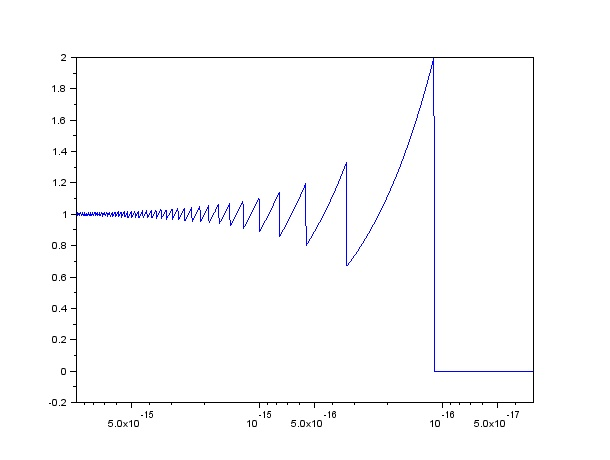
\includegraphics[width=0.8\textwidth]{./cap_aritmetica/pics/cancelamento_0}  
  \caption{Oi. Eu estou aqui!}
  \label{fig:cancelamento_0}
\end{figure}

\end{ex}

\begin{ex} Neste exemplo, estamos interessados em compreender mais detalhadamente o comportamento da expressão
\begin{equation}\label{def_lim}\left(1+\frac{1}{n}\right)^n\end{equation}
quando $n$ é um número grande ao computá-la em sistemas de numeral de ponto flutuante com acurácia finita.
Um resultado bem conhecido do cálculo nos diz que o limite de (\ref{def_lim}) quando $n$ tende a infinito é o número de Euler:
\begin{equation}\label{lim}\lim_{n\to \infty}\left(1+\frac{1}{n}\right)^n=e= 2,718281828459...\end{equation}

Sabemos também que a sequência produzida por (\ref{def_lim}) é crescente, isto é:
$$\left(1+\frac{1}{1}\right)^1< \left(1+\frac{1}{2}\right)^2< \left(1+\frac{1}{3}\right)^3 < \cdots $$

No entanto, quando calculamos essa expressão no \verb+Scilab+, nos defrontamos com o seguinte resultado:
$$\begin{array}{|c|c|c|c|c|}
\hline &&&&\\[-0.3cm]
n & \left(1+\frac{1}{n}\right)^n&~~~~&n & \left(1+\frac{1}{n}\right)^n\\
 &&&&\\[-0.3cm]
\hline\\[-0.3cm]
1 & 2,0000000000000 && 10^{2} & 2,7048138294215 \\
2 & 2,2500000000000 && 10^{4} & 2,7181459268249 \\
3 & 2,3703703703704 && 10^{6} & 2,7182804690957 \\
4 & 2,4414062500000 && 10^{8} & 2,7182817983391 \\
5 & 2,4883200000000 && 10^{10} & 2,7182820532348 \\
6 & 2,5216263717421 && 10^{12} & 2,7185234960372 \\
7 & 2,5464996970407 && 10^{14} & 2,7161100340870 \\
8 & 2,5657845139503 && 10^{16} & 1,0000000000000 \\
9 & 2,5811747917132 && 10^{18} & 1,0000000000000 \\
10 & 2,5937424601000 && 10^{20} & 1,0000000000000 \\
\hline
\end{array}
$$
Podemos resumir esses dados no seguinte gráfico de $\left(1+\frac{1}{n}\right)^n$ em função de $n$:

%\begin{figure}[htp]
\includegraphics[width=0.8\textwidth]{./cap_aritmetica/pics/cancelamento_euler.eps}
%\caption{Gráfico de $\left(1+\frac{1}{n}\right)^n$ em função de $n$ em escala linear-logarítmica variando de $10^0$ até $10^{18}$ gerado no Scilab 5.4.1.}
%\end{figure}

Observe que quando $x$ se torna grande, da ordem de $10^{15}$, o gráfico da função deixa de se crescente e apresenta oscilações.  Observe também que a expressão se torna identicamente igual a $1$ depois de um certo limiar. Tais fenômenos não são intrínsecos da função $f(x)=(1+1/x)^x$, mas \emph{\uline{oriundas de erros de arredondamento}}, isto é, são resultados numéricos espúrios. A fim de pôr o comportamento numérico de tal expressão, apresentamos abaixo o gráfico da mesma função, porém restrito à região entre $10^{14}$ e $10^{16}$.

%\begin{figure}
\includegraphics[width=0.9\textwidth]{./cap_aritmetica/pics/cancelamento_euler2.eps}
%\caption{Gráfico de $\left(1+\frac{1}{n}\right)^n$ em função de $n$ em escala linear-logarítmica variando de $10^{14}$ até $10^{16}$ gerado no Scilab 5.4.1.}
¨%\end{figure}
\end{ex}

Para compreendermos melhor por que existe um limiar $N$ que, quando atingido torna a expressão do exemplo acima identicamente igual a $1$, observamos a sequência de operações realizadas pelo computador:
\begin{equation}\label{seq_oper}
x~\to ~1/x ~\to ~1+1/x ~\to ~(1+1/x)^x
\end{equation}
Devido ao limite de precisão da representação de números em ponto flutuante, existe um menor número representável que é maior do que 1. Este número é $1 + $\verb+eps+, onde \verb+eps+ é chamado de \emph{épsilon de máquina} e é o menor número que somado a 1 produz um resultado superior a 1 no sistema de numeração usado. O épsilon de máquina no sistema de numeração \emph{double} vale aproximadamente $2,22\times 10^{-16}$.
\ifisscilab
No \verb+Scilab+, o epsilon de máquina é a constante \verb+eps+. Observe que:
\begin{verbatim}
-->1+%eps
 ans  =
    1.0000000000000002220446 
\end{verbatim}
\fi
Quando somamos a $1$ um número positivo inferior ao épsilon de máquina, obtemos o número 1. Dessa forma, o resultado obtido pela operação de ponto flutuante $1+x$ para $0<x<2,22 \times 10^{-16}$ é 1. 

Portanto, quando realizamos a sequência de operações dada em (\ref{seq_oper}), toda informação contida no número $x$ é perdida na soma com $1$ quando $1/x$ é menor que o épsilon de máquina, o que ocorre quando $x>5\times 10^{15}$. Assim $(1+1/x)$ é aproximado para $1$ e a última operação se resume a $1^x$, o que é igual a $1$ mesmo quando $x$ é grande.

Um erro comum é acreditar que o perda de significância se deve ao fato de $1/x$ ser muito pequeno para ser representado e é aproximando para $0$. Isto é falso, o sistema de ponto de flutuante permite representar números de magnitude muito inferior ao épsilon de máquina. O problema surge da limitação no tamanho da mantissa. Observe como a seguinte sequência de operações não perde significância para números positivos x muito menores que o épsilon de máquina:
\begin{equation}\label{seq_oper2}
x ~\to ~1/x ~\to ~1/(1/x) 
\end{equation}
 compare o desempenho numérico desta sequência de operações para valores pequenos de $x$ com o da seguinte sequência:
\begin{equation}\label{seq_oper3}
x ~\to ~1+x ~\to ~(1+x)-1.
\end{equation}
Finalmente, notamos que quando tentamos calcular $\left(1+\frac{1}{n}\right)^n$ para $n$ grande, existe perda de significância no cálculo de $1+1/n$. 
\ifisscilab
Para entendermos isso melhor, vejamos o que acontece no \verb+Scilab+ quando $n=7\times 10^{13}$:
\begin{verbatim}
-->n=7e13
 n  =
     7.000000000000000000D+13  
 
-->1/n
 ans  =
     1.428571428571428435D-14  
 
-->y=1+1/n
 y  =
 
    1.000000000000014211D+00  
\end{verbatim}
Observe a perda de informação ao deslocar a mantissa de $1/n$. Para evidenciar o fenômenos, observamos o que acontece quando tentamos recalcular $n$ subtraindo $1$ de $1+1/n$ e invertendo o resultado:
\begin{verbatim}
-->y-1
 ans  =
     1.421085471520200372D-14  
 
-->1/(y-1)
 ans  =
     7.036874417766400000D+13  
\end{verbatim}
\fi

\begin{ex}[Analogia da balança] Observe a seguinte comparação interessante que pode ser feita para ilustrar os sistemas de numeração com ponto fixo e flutuante: o sistema de ponto fixo é como uma balança cujas marcas estão igualmente espaçadas; o sistema de ponto flutuante é como uma balança cuja distância entre as marcas é proporcional à massa medida. Assim, podemos ter uma balança de ponto fixo cujas marcas estão sempre distanciadas de $100$g ($100$g, $200$g, $300$g, ..., $1$Kg, $1,1$Kg,...) e outra balança de ponto flutuante cujas marcas estão distanciadas sempre de aproximadamente um décimo do valor lido ($100$g, $110$g, $121$g, $133$g, ..., $1$Kg, $1,1$Kg, $1,21$Kg, ...) A balança de ponto fixo apresenta uma resolução baixa para pequenas medidas, porém uma resolução alta para grandes medidas. A balança de ponto flutuante distribui a resolução de forma proporcional ao longo da escala.    

Seguindo nesta analogia, o fenômeno de perda de significância pode ser interpretado como a seguir: imagine que você deseje obter o peso de um gato (aproximadamente $4$Kg). Dois processos estão disponíveis: colocar o gato diretamente na balança ou medir seu peso com o gato e, depois, sem o gato. Na balança de ponto flutuante, a incerteza associada na medida do peso do gato (sozinho) é aproximadamente $10\%$ de $4$Kg, isto é, $400$g. Já a incerteza associada à medida da uma pessoa (aproximadamente $70$Kg) com o gato é de $10\%$ do peso total, isto é, aproximadamente $7$Kg. Esta incerteza é da mesma ordem de grandeza da medida a ser realizada, tornado o processo impossível de ser realizado, já que teríamos uma incerteza da ordem de $14$Kg (devido à dupla medição) sobre uma grandeza de $4$Kg.    
\end{ex}

\subsection{Exercícios}

\begin{Exercise} Considere as expressões:
  \begin{equation*}
    \frac{\exp(1/\mu)}{1+\exp(1/\mu)}  
  \end{equation*}
e
\begin{equation*}
  \frac{1}{\exp(-1/\mu)+1}
\end{equation*}
com $\mu>0$. Verifique que elas são idênticas como funções reais. Teste no computador cada uma delas para $\mu=0,1$, $\mu=0,01$ e $\mu=0,001$. Qual dessas expressões é mais adequada quando $\mu$ é um número pequeno? Por quê?
\end{Exercise}
\begin{Answer}
  \begin{tiny}
  Quando $\mu$ é pequeno, $e^{1/mu}$ é um número grande. A primeira expressão produz um ''overflow'' (número maior que o máximo representável) quando $\mu$ é pequeno. A segunda expressão, no entanto, reproduz o limite $1$ quando $\mu\to 0+$.
  \end{tiny}
\end{Answer}

\begin{Exercise} Encontre expressões alternativas para calcular o valor das seguintes funções quando $x$ é próximo de zero.
\begin{itemize}
\item[a)] $f(x)=\frac{1-\cos(x)}{x^2}$
\item[b)] $g(x)=\sqrt{1+x}-1$
\item[c)] $h(x)=\sqrt{x+10^6}-10^3$
\item[d)] $i(x)=\sqrt{1+e^{x}}-\sqrt{2}$ ~~~~~~ Dica: Faça $y=e^{x}-1$
\end{itemize}
\end{Exercise}
\begin{Answer}
  \begin{tiny}
    a)~$\frac{1}{2}+\frac{x^2}{4!}+O(x^4)$; b)~$x/2+O(x^2)$; c)~$5\cdot 10^{-4}x+O(x^2)$; d)~$\frac{\sqrt{2}}{4}y+O(y^{2})=\frac{\sqrt{2}}{4}x+O(x^2)$
  \end{tiny}
\end{Answer}

\begin{Exercise} Use uma identidade trigonométrica adequada para mostrar que:
  \begin{equation*}
    \frac{1-\cos(x)}{x^2}= \frac{1}{2} \left(\frac{\sin(x/2)}{x/2}\right)^2.
  \end{equation*}
Analise o desempenho destas duas expressões no computador quando $x$ vale $10^{-5}$, $10^{-6}$, $10^{-7}$, $10^{-8}$, $10^{-9}$, $10^{-200}$ e $0$. Discuta o resultado.
\emph{Dica:} Para $|x|<10^{-5}$, $f(x)$ pode ser aproximada por $1/2-x^2/24$ com erro de truncamento inferior a $10^{-22}$.
\end{Exercise}

%\begin{Exercise} Considere a expressão
%$$
%f(x)=\frac{1-\cos(x)}{x^2}
%$$
%para $x$ pequeno. Verifique que
%$$
%\lim_{x\to 0}f(x)=0,5
%$$
%Depois calcule no \verb+Scilab+ $f(x)$ para $x=10^{-5}$, $x=10^{-6}$, $x=10^{-7}$, $x=10^{-8}$, $x=10^{-9}$ e $x=10^{-10}$. Finalmente, faça uma %aproximação analítica que elimine o efeito catastrófico.
%\end{Exercise}
%%Redundante


\begin{Exercise}[title=Notas do prof. Guidi] Reescreva as expressões:
  $$\sqrt{e^{2x}+1}-e^x \qquad\hbox{e}\qquad \sqrt{e^{2x}+x^2}-e^x $$
  de modo que seja possível calcular seus valores para $x=100$ utilizando a aritmética de ponto flutuante ("Double") no computador.
\end{Exercise}

\begin{Exercise} Na teoria da relatividade restrita, a energia cinética de uma partícula e sua velocidade se relacionam pela seguinte fórmula:
  \begin{equation*}
    E=mc^2\left(\frac{1}{\sqrt{1-(v/c)^2}}-1\right),
  \end{equation*}
onde $E$ é a energia cinética da partícula, $m$ é a massa de repouso, $v$ o módulo da velocidade e $c$ a velocidade da luz no vácuo dada por $c=299792458 m/s$. Considere que a massa de repouso $m=9,10938291\times 10^{-31} Kg$ do elétron seja conhecida com erro relativo de $10^{-9}$. Qual é o valor da energia e o erro relativo associado a essa grandeza quando $v=0,1 c$, $v=0,5 c$, $v=0,99c$ e $v=0,999c$ sendo que a incerteza relativa na medida da velocidade é $10^{-5}$?
\end{Exercise}
\begin{Answer}
  \begin{tiny}
    $4,12451228\times 10^{-16}$~J; $0,002\%$; $0,26654956\times 10^{-14}$~J; $0,002\%$; $4,98497440\times 10^{-13}$~J; $0,057\%$; $1,74927914\times 10^{-12}$~J; $0,522\%$.
  \end{tiny}
\end{Answer}

\begin{Exercise} Deseja-se medir a concentração de dois diferentes oxidantes no ar. Três sensores eletroquímicos estão disponíveis para a medida e apresentam a seguintes respostas:
$$v_1= 270 [A] +  30 [B],~~~ v_2= 140 [A] +  20 [B] ~~ \hbox{e}~~ v_3= 15 [A] +  200 [B]$$
as tensões $v_1$, $v_2$ e $v_3$ são dadas em $mV$ e as concentrações em $milimol/l$.
\begin{itemize}
\item [a)] Encontre uma expressão para os valores de $[A]$ e $[B]$ em termos de $v_1$ e $v_2$ e, depois, em termos de $v_1$ e $v_3$. Dica:
Se $ad\neq bc$, então a matriz $A$ dada por
$$A=\left[\begin{array}{cc}a&b\\c&d\end{array}\right]$$
é inversível e sua inversa é dada por
$$A^{-1}= \frac{1}{ad-bc} \left[\begin{array}{cc}d&-b\\-c&a\end{array}\right].$$

\item[b)] Sabendo que incerteza relativa associada às sensibilidades dos sensores 1 e 2 é de $2\%$ e que a incerteza relativa associada às sensibilidades do sensor 3 é $10\%$, verifique a incerteza associada à medida feita com o par $1-2$ e o par $1-3$. Use $[A]=[B]=10milimol/l$. Dica: Você deve diferenciar as grandezas $[A]$ e $[B]$ em relação aos valores das tensões.
\end{itemize}
\end{Exercise}
\begin{Answer}
  \begin{tiny}
Em ambos casos, temos a seguinte estrutura:
$$\left[\begin{array}{cc}
S_{11}& S_{12}\\
S_{21}& S_{22}
\end{array}
\right] \left[\begin{array}{c}
\left[ A\right]\\
\left[ B\right]
\end{array}
\right]= \left[\begin{array}{c}
v_1\\
v_2
\end{array}
\right]$$
De forma que
$$ \left[\begin{array}{c}
\left[ A\right]\\
\left[ B\right]
\end{array}\right]
=\left[\begin{array}{cc}
S_{11}& S_{12}\\
S_{21}& S_{22}
\end{array}
\right]^{-1}
\left[\begin{array}{c}
v_1\\
v_2
\end{array}
\right]=\frac{1}{S_{11}S_{22}-S_{12}S_{21}}\left[\begin{array}{cc}
S_{22}& -S_{12}\\
-S_{21}& S_{11}
\end{array}
\right]\left[\begin{array}{c}
v_1\\
v_2
\end{array}
\right]
$$
Portanto
\begin{eqnarray*}
[ A ]&=&\frac{S_{22}v_1-S_{12}v_2}{S_{11}S_{22}-S_{12}S_{21}}\\
\left[ {B} \right]&=&\frac{-S_{21}v_1+S_{11}v_2}{S_{11}S_{22}-S_{12}S_{21}}
\end{eqnarray*}

Usando derivação logarítmica, temos

\begin{eqnarray*}
\frac{1}{[ A ]}\frac{\partial [ A ]}{\partial S_{11}}&=&-\frac{S_{22}}{S_{11}S_{22}-S_{12}S_{21}}\\
\frac{1}{[ A ]}\frac{\partial [ A ]}{\partial S_{12}}&=&-\frac{v_2}{S_{22}v_1-S_{12}v_2}+\frac{S_{21}}{S_{11}S_{22}-S_{12}S_{21}}=-\frac{[A]}{\left[B\right]}\cdot \frac{S_{22}}{S_{11}S_{22}-S_{12}S_{21}}\\
\frac{1}{[ A ]}\frac{\partial [ A ]}{\partial S_{21}}&=&\frac{S_{12}}{S_{11}S_{22}-S_{12}S_{21}}\\
\frac{1}{[ A ]}\frac{\partial [ A ]}{\partial S_{22}}&=&\frac{v_1}{S_{22}v_1-S_{12}v_2}-\frac{S_{11}}{S_{11}S_{22}-S_{12}S_{21}}=\frac{[A]}{\left[B\right]}\cdot \frac{S_{12}}{S_{11}S_{22}-S_{12}S_{21}}
\end{eqnarray*}
e
\begin{eqnarray*}
\frac{1}{\left[ B \right]}\frac{\partial \left[ B \right]}{\partial S_{11}}&=&\frac{v_2}{-S_{21}v_1+S_{11}v_2}-\frac{S_{22}}{S_{11}S_{22}-S_{12}S_{21}}=\frac{\left[B\right]}{[A]} \frac{S_{21}}{S_{11}S_{22}-S_{12}S_{21}}\\
\frac{1}{\left[ B \right]}\frac{\partial \left[ B \right]}{\partial S_{12}}&=&\frac{S_{21}}{S_{11}S_{22}-S_{12}S_{21}}\\
\frac{1}{\left[ B \right]}\frac{\partial \left[ B \right]}{\partial S_{21}}&=&-\frac{v_1}{-S_{21}v_1+S_{11}v_2}+\frac{S_{21}}{S_{11}S_{22}-S_{12}S_{21}}=-\frac{\left[B\right]}{[A]}\frac{S_{11}}{S_{11}S_{22}-S_{12}S_{21}}\\
\frac{1}{\left[ B \right]}\frac{\partial \left[ B \right]}{\partial S_{22}}&=&-\frac{S_{11}}{S_{11}S_{22}-S_{12}S_{21}}\\
\end{eqnarray*}


E o erro associado às medidas pode ser aproximado por
\begin{eqnarray*}
\frac{1}{[A]}\delta_{[A]}&=&\left|\frac{1}{[ A ]}\frac{\partial [ A ]}{\partial S_{11}}\right| \delta_{S_{11}}+\left|\frac{1}{[ A ]}\frac{\partial [ A ]}{\partial S_{12}}\right| \delta_{S_{12}}+\left|\frac{1}{[ A ]}\frac{\partial [ A ]}{\partial S_{21}}\right| \delta_{S_{21}}+\left|\frac{1}{[ A ]}\frac{\partial [ A ]}{\partial S_{22}}\right| \delta_{S_{22}}\\
&=&\frac{1}{\left|\det{S}\right|}\left[S_{22}\delta_{S_{11}}+\frac{[A]}{\left[B\right]}S_{22}\delta_{S_{12}}+S_{12}\delta_{S_{21}}+\frac{[A]}{\left[B\right]}S_{12}\delta_{S_{22}}\right]
\end{eqnarray*}
Analogamente, temos:
\begin{eqnarray*}
\frac{1}{[B]}\delta_{[B]}&=&\frac{1}{\left|\det{S}\right|}\left[\frac{[B]}{\left[A\right]}S_{21}\delta_{S_{11}}+S_{21}\delta_{S_{11}}+\frac{\left[B\right]}{[A]}S_{11}\delta_{S_{21}}+S_{11}\delta_{S_{22}}\right]
\end{eqnarray*}

onde não se indicou $|S_{ij}|$ nem $|[.]|$ pois são todos positivos.


Fazemos agora a aplicação numérica:

{\bf Caso do par 1-2:}
$$\det{S}=\left|\begin{array}{cc}270&30\\140&20\end{array}\right|=1200$$
\begin{eqnarray*}
\frac{1}{[A]}\delta_{[A]}
&=&\frac{1}{1200}\left[20\times 270\times 2\%+20\times 30\times 2\%+30\times 140\times 2\%+30\times 20\times 2\%\right]\\&=&\frac{216}{1200}=0.18=18\%\\
\frac{1}{[B]}\delta_{[B]}
&=&\frac{1}{1200}\left[140\times 270\times 2\%+140\times 30\times 2\%+270\times 140\times 2\%+270\times 20\times 2\%\right]\\&=&\frac{426}{1200}=0.355=35.5\%
\end{eqnarray*}

{\bf Caso do par 1-3:}
$$\det{S}=\left|\begin{array}{cc}270&30\\15&200\end{array}\right|=53550$$
\begin{eqnarray*}
\frac{1}{[A]}\delta_{[A]}
&=&\frac{1}{53550}\left[200\times 270\times 2\%+200\times 30\times 2\%+30\times 15\times 10\%+30\times 200\times 10\%\right]\\&=&\frac{1804,6}{52550}\approx 0.0337=3.37\%\\
\frac{1}{[B]}\delta_{[B]}
&=&\frac{1}{53550}\left[15\times 270\times 2\%+15\times 30\times 2\%+270\times 15\times 10\%+270\times 200\times 10\%\right]\\&=&	\frac{5895}{53550}\approx   0.11=11\%
\end{eqnarray*}

Conclusão, apesar de o sensor $3$ apresentar uma incerteza cinco vezes maior na sensibilidade, a escolha do sensor $3$ para fazer par ao sensor $1$ parece mais adequada.    
  \end{tiny}
\end{Answer}

%\end{document} 
